\documentclass{standalone}
\usepackage{tikz}
\usetikzlibrary{positioning}
\usetikzlibrary{fit}
\usetikzlibrary{shapes,snakes}
\usetikzlibrary{arrows,automata}
\usepackage{amsmath}
\usepackage{booktabs}
\usepackage{array}
\usepackage{eulervm}
\usepackage{inconsolata}
\usepackage{graphicx,amssymb}
\usepackage{stmaryrd}
\tikzset{every initial by arrow/.style={*->},every initial by text/.style={ }}
\begin{document}
	
\begingroup\renewcommand\arraystretch{1.3}
\newcommand{\lefto}{\rotatebox[origin=c]{-135}{\xleftarrow{\quad\texttt{nmod}\quad}}}
\noindent
\renewcommand{\arraystretch}{1.5}
\begin{tabular}{| *2{>{\centering\arraybackslash}m{2.5in}|} @{}m{0pt}@{}}
	\toprule
	\textbf{Pattern} & \textbf{Result} \\
	\midrule
	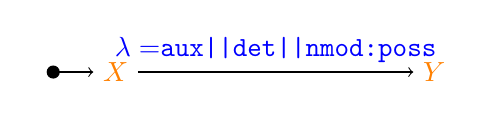
\begin{tikzpicture}
	\node[label] (start) at (-1,0) {};
	\node (X) {\color{orange}$X$}; \node[right=of X] (Q) {}; \node[right=of Q] (Z) {};\node[right=of Z] (Y) {\color{orange}$Y$}; \draw[->] (X) -- node[above,sloped] {\color{blue}$\lambda=$\texttt{aux||det||nmod:poss}} (Y);
	\draw[*->] (start) -- (X);
	\end{tikzpicture} & 
	\textbf{move} $\color{orange}Y$ \textbf{in} ${\color{orange}X} @ \{{\color{blue}\lambda}\colon {\color{orange}Y.value}\}$\\
	\hline
	
%	\begin{tikzpicture}
%	\node[label] (start) at (-0.8,0) {};
%	\node (X) {\color{orange}$X$}; \node[right=of X] (Q) {}; \node[right=of Q] (Y) {\color{orange}$\mathbf{X}||V$}; \draw[->] (X) -- node[above,sloped] {\color{blue}\texttt{acl:recl}} (Y);
%	\draw[*->] (start) -- (X);
%	\end{tikzpicture} & 
%	\begin{tikzpicture}
%		\node[label] (start) at (-0.8,0) {};
%		\node (X) {\color{orange}$X$}; \node[right=of X] (Q) {}; \node[right=of Q] (Y) {\color{orange}$\mathbf{X}||V$}; \draw[->] (X) -- node[above,sloped] {\color{blue}\texttt{acl:recl}} (Y);
%		\draw[*->] (start) -- (X);
%	\end{tikzpicture}\\
%	\hline
	
%	\begin{tikzpicture}
%	\node (X) {$\color{orange}X$}; \node[right=of X] (Y) {$\color{orange}Y$}; \node[right=of Y] (Z) {$\color{orange}Z$}; \draw[->] (X) -- node[above,sloped] {\color{blue}\texttt{nmod}} (Y); \draw[->] (Y) -- node[above,sloped] {\color{blue}\texttt{case}} (Z);
%	\end{tikzpicture} & 
%	\begin{tikzpicture}
%	\node (X) {$\color{orange}X$}; \node[right=of X] (ii) {}; \node[right=of ii] (Y) {${\color{orange}Y}$}; \draw[->] (X) -- node[above,sloped] {\texttt{complement($\color{orange}Z$)}} (Y);
%	\end{tikzpicture}\\
%	\hline
	
	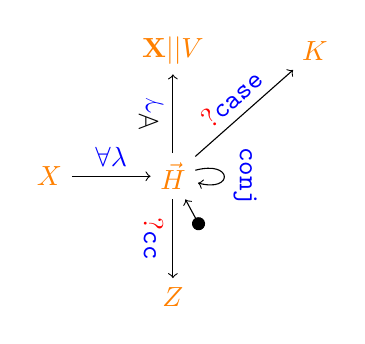
\begin{tikzpicture}
		\node (X) {$\color{orange}X$};
		\node[right=of X] (Y1) {$\color{orange}\vec{H}$};
		\node[below=of Y1] (Z) {$\color{orange}Z$};
		\node[above=of Y1] (T) {\color{orange}$\mathbf{X}||{V}$};
		\node[right=of T] (K) {$\color{orange}K$};
		\node (start) at (2,-0.8) {};
		\draw[*->] (start) -- (Y1);
		\draw[->] (X) -- node[above,sloped] {\color{blue}$\forall\lambda$} (Y1);
		\draw[->] (Y1) edge[loop right] node[above,sloped] {\color{blue}\texttt{conj}} (); 
		\draw[->] (Y1) -- node[below,sloped] {\color{red}?\color{blue}\texttt{cc}} (Z); 
		\draw[->] (Y1) -- node[above,sloped] {$\forall$\color{blue}$\gamma$} (T); 
		\draw[->] (Y1) -- node[above,sloped] {\color{red}?\color{blue}\texttt{case}} (K);
	\end{tikzpicture} & 
	\textbf{let} $\color{blue}\tilde{\lambda}$ \textbf{:= if} ${\color{blue}\lambda}=$\texttt{nmod} \textbf{then} $complement({\color{orange}K})$ \textbf{else} ${\color{blue}\lambda}$ \textbf{in}
	
	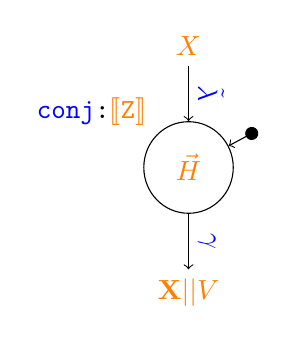
\begin{tikzpicture}
	\node (X) {$\color{orange}X$};
	\node[below     =of X] (Yn) {$\color{orange}\vec{H}$};
	\node[below     =of Yn] (T) {\color{orange}$\mathbf{X}||{V}$};
	\node[fit=(Yn),ellipse,draw=black,label=above left:{
		\texttt{{\color{blue}conj}:{\color{orange}$\llbracket$Z$\rrbracket$}}}] (Y12) {};
		\node (start) at (1,-1) {};
		\draw[*->] (start) -- (Y12);
	%\draw[->] (Y1) -- coordinate[midway] (MW) node[above,sloped] {\texttt{{\color{blue}conj}:{\color{orange}Z}}} (Y2); 
	\draw[->] (X) -- node[above,sloped] {$\color{blue}\tilde{\lambda}$} (Y12);
	\draw[->] (Y12) -- node[above,sloped] {$\color{blue}\gamma$} (T);
	\end{tikzpicture} \\
	\hline
	
	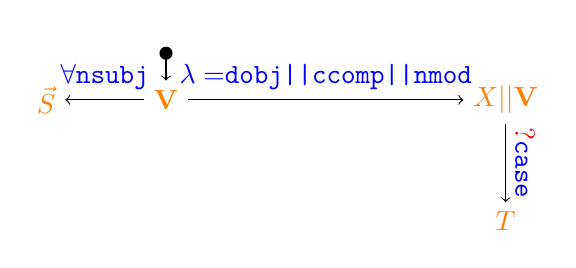
\begin{tikzpicture}
	\node (X) {$\color{orange}\mathbf{V}$};
	\node at (0,0.8) (start) {};
	\draw[*->] (start) -- (X);
	
	\node[left=of X] (Y1) {$\color{orange}\vec{S}$};
	\node[right=of X] (U) {};
	\node[right=of U] (Y) {};
	\node[right=of Y] (Y2) {$\color{orange}X||\mathbf{V}$};
	\node[below=of Y2] (T) {$\color{orange}T$};
	\draw[->] (Y2) -- node[above,sloped] {\color{red}?\color{blue}\texttt{case}} (T);
	\draw[->] (X) -- node[above,sloped] {\color{blue}$\forall$\texttt{nsubj}} (Y1);
	\draw[->] (X) -- node[above,sloped] {\color{blue}$\lambda=$\texttt{dobj||ccomp||nmod}} (Y2);
	\end{tikzpicture} & 
	
\textbf{let} $\color{blue}\tilde{\lambda}$ \textbf{:= if} ${\color{blue}\lambda}=$\texttt{nmod} \textbf{then} $complement({\color{orange}T})$ \textbf{else} $\color{orange}\llbracket V\rrbracket$ \textbf{in}
	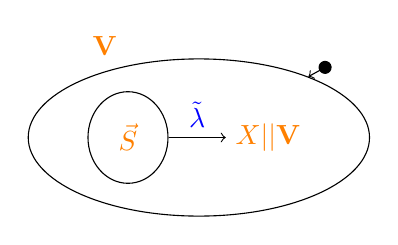
\begin{tikzpicture}
	\node (X) {$\color{orange}\vec{S}$}; \node[fit=(X),ellipse,draw=black] (f) {};\node[right=of X] (Y) {\color{orange}$X||\mathbf{V}$}; \draw[->] (f) -- node[above,sloped] {\color{blue}$\tilde{\lambda}$} (Y);
	\node[fit=(f)(Y),draw=black,ellipse,label=above left:{\color{orange}$\mathbf{V}$}] (VAbove) {};
		\node (start) at (2.7,1) {};
		\draw[*->] (start) -- (VAbove);
	\end{tikzpicture} \\
	\hline
	
%	\begin{tikzpicture}
%	\node (X) {$\color{orange}V$};
%	\node[below left=of X] (Y1) {$\color{orange}\vec{S}$};
%	\node[below right=of X] (Y2) {$\color{orange}O$};
%	\draw[->] (X) -- node[above,sloped] {\color{blue}$\forall$\texttt{nsubj}} (Y1);
%	\draw[->] (X) -- node[above,sloped] {\color{blue}\texttt{dobj}} (Y2);
%	\end{tikzpicture} & 
%	\begin{tikzpicture}
%	\node (X) {$\color{orange}\vec{S}$}; \node[fit=(X),ellipse,draw=black] (f) {};\node[right=of X] (Y) {\color{orange}$O$}; \draw[->] (f) -- node[above,sloped] {\color{orange}$V$} (Y);
%	\end{tikzpicture} \\
	\bottomrule
\end{tabular}
\endgroup

\end{document}